\documentclass[handout]{beamer}
% \usepackage[utf8]{inputenc}
\usepackage{polski}
% \usepackage[polish]{babel}
\usepackage[T1]{fontenc}
\usepackage{tikz}
\usepackage{tikzducks}
% \usetikzlibrary{decorations.pathmorphing}
\usepackage{multimedia}
\usepackage{graphicx}
\usepackage[justification=centering]{caption}
\usepackage{textcomp}
\usepackage{appendixnumberbeamer}
\usepackage{qrcode}
% \usepackage[natbib, language=polish, sorting=none]{biblatex}
% \addbibresource{lio.bib}
\usepackage{hyperref}
%\usepackage[width=\textwidth]{animate}
%\usepackage{chemformula}
% \usepackage{sidecap}
\usepackage{multirow}
\usepackage{rotating}
\usepackage{anyfontsize} % change font size for semposiwko

\usepackage{listings}
\lstset{
basicstyle=\small\ttfamily,
columns=flexible,
breaklines=true
}

\usepackage{emoji}
    \usepackage{bredzenie}
    \usepackage{wrapfig}
\graphicspath{ {./memy/}{./} }
\usepackage{subcaption}
\usepackage[rightcaption]{sidecap}
% \usepackage{float}



\usepackage[natbib, language=polish, sorting=none]{biblatex}
\addbibresource{lio.bib}
\renewcommand*{\bibfont}{\scriptsize}

\usetheme{Szeged}
\usecolortheme{whale}
\setbeamercolor{palette primary}{bg=violet!80!black,fg=white}
\setbeamercolor{palette secondary}{bg=violet!60!black,fg=white}
\setbeamercolor{palette tertiary}{bg=violet!40!black,fg=white}
\setbeamercolor{palette quaternary}{bg=violet!20!black,fg=white}
\setbeamercolor{structure}{fg=violet!60!black}
\setbeamertemplate{caption}{\insertcaption}
% \setbeamertemplate{headline}{
%   \begin{beamercolorbox}[wd=.9\paperwidth]{headline}
%     \vspace{1.5ex}
%     \insertsectionnavigationhorizontal
%     \vspace{1.5ex}
%   \end{beamercolorbox}
% }

\linespread{0.6}

\setbeamertemplate{background}%
{%
    \begin{tikzpicture}[remember picture,overlay]{\node[yshift=1.5cm,xshift=-2cm,opacity=0.1] at (current page.south east)
      {
      \includegraphics[scale=0.4, angle=20]{ptaki.pdf}
      }
      ;
    \node[yshift=1.0cm,xshift=0.6cm] (logopos) at (current page.south west) {{\begin{tikzpicture}\shuffleducks\duck[signpost=\insertframenumber, \randomhead,scale=.4]\end{tikzpicture}}};
    \pgfmathsetmacro{\progress}{360*(\insertframenumber)/(\inserttotalframenumber)};
    \draw[line width=0.2*3pt] ([xshift=0.55cm] logopos)  arc[radius=0.55cm, start angle=0, end angle=\progress];
    \fill ([shift={(\progress:0.55cm)}] logopos) circle(1pt);

    }
        \end{tikzpicture}
    
}

\newcommand{\SeMPowisko}{%
\large S\normalsize%
\kern-.3em \lower.2ex\hbox{e}%
\lower.2ex\hbox{\large M\normalsize}%
\kern-.1em \raise.1ex\hbox{\large P\normalsize}%
\kern-.3em \lower.2ex\hbox{o}%
\kern-.2em \raise.2ex\hbox{w}%
\lower.2ex\hbox{i}%
s%
\raise.2ex\hbox{k}%
\kern-.3em \lower.2ex\hbox{o}%
}

\newcommand\Tikz{Ti\emph{k}Z}

% \makeatletter
% \def\beamer@startmycovered{%
%   \def\opaqueness<##1>##2{%
%     \only<##1>{%
%       \beamer@actions{%
%         \expandafter\xdef\csname beamer@oldcolorhook%
%         \the\beamer@coveringdepth\endcsname{\beamer@colorhook}%
%         \expandafter\xdef\csname beamer@oldpgfextension%
%         \the\beamer@coveringdepth\endcsname{\beamer@pgfextension}%
%         {\globalcolorstrue\colorlet{beamer@freeze\the\beamer@coveringdepth}{bg}}%
%         \xdef\beamer@colorhook{!##2!beamer@freeze%
%           \the\beamer@coveringdepth\beamer@colorhook}%
%         \gdef\beamer@pgfextension{!##2opaque}%
%         \color{.}%
%       }%
%       {%
%         \xdef\beamer@colorhook{\csname beamer@oldcolorhook%
%           \the\beamer@coveringdepth\endcsname}%
%         \xdef\beamer@pgfextension{\csname beamer@oldpgfextension%
%           \the\beamer@coveringdepth\endcsname}%
%         \color{.}%
%       }}}%
%   \ifnum\beamer@slideinframe<\beamer@minimum%ok, at beginning
%   {%
%     \beamer@saveanother%
%     \advance\beamer@minimum by-\beamer@slideinframe%
%     \beamer@slideinframe=\beamer@minimum%
%     \beamer@uncoverbeforeactions%
%     \beamer@restoreanother%
%   }%
%   \else%
%   {%
%     \beamer@saveanother%
%     \advance\beamer@slideinframe by-\beamer@minimum%
%     \beamer@uncoverafteractions%
%     \beamer@restoreanother%
%   }%
%   \fi%
%   \beamer@do%
% %  }%
% }

% \long\def\beamer@makemycovered#1{\beamer@startmycovered#1\beamer@endcovered}
% \def\mycover{%
% \alt{\beamer@makemycovered}{\beamer@fakeinvisible}}
% \def\c@slideinframe{\beamer@slideinframe}
% \makeatother

% \setbeamercovered{transparent} % jestem pewien że da się to zrobić ładniej, za https://tex.stackexchange.com/a/171320

\newcommand{\tb}{\textbackslash}

\title{Wstawianie gra\varphi{}ki}
\subtitle{od zera do Worda}
\author[M. Winiarski]{Mateusz (czarny) Winiarski}
\institute[KMPS UJ]{KMPS UJ, WFAIS}
\date[dzisiaj]{dzisiaj}

\begin{document}

\section{In}
\frame{\titlepage}

\begin{frame}{Ostrzeżenie}{}
\begin{itemize}[<+->]
    \item \LaTeX{} to oprogramowanie do zautomatyzowanego składu tekstu...
    \item ...co oznacza, że jak \LaTeX{} bardzo dobrze wie, gdzie wstawić obrazek...
    \item ...i wstawienie go \emph{dokładnie} tak, jak chcesz może być trudne.
\end{itemize}    
\end{frame}

\section{the}

\begin{frame}{Jak wstawić rysunek w Wordzie?}
\Large
\begin{itemize}[<+->]
    \item Krok 1: \texttt{Ctrl}+\texttt{V}
    \item Krok 2: \emoji{sob}
    \item Ekskomunika z kościoła kopistów
\end{itemize}
    
\end{frame}

\begin{frame}{Jak wstawić rysunek w Overleafie?}
\Large
Uwierz mi lub nie:
\begin{itemize}[<+->]
    \item Krok 1: \texttt{Ctrl}+\texttt{V}
    \item Krok 2: \emoji{smiling-face-with-sunglasses}
    \item Najlepszy wynalazek od czasu krojonego chleba
\end{itemize}

\only<3->{\begin{figure}
    \centering
    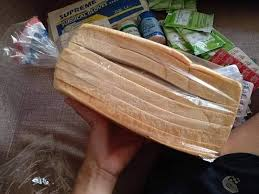
\includegraphics[width=0.5\textwidth]{mem1.jpg}
\end{figure}}
    
\end{frame}

\setbeamercovered{transparent}
\begin{frame}[fragile]{No dobra Mateusz, ale co ja zrobiłem przed chwilą?}
\setbeamercovered{transparent}

% \only<2->{\texttt{test}}

\uncover<1,2>{\texttt{\textbackslash{}begin\{figure\}}}

\uncover<1,3>{\texttt{
    \textbackslash centering
}}

\uncover<1,4>{\texttt{
    \textbackslash includegraphics[width=0.5\textbackslash linewidth]\{image.png\}
}}

\uncover<1,5>{\texttt{
    \textbackslash caption\{Enter Caption\}
}}

\uncover<1,6>{\texttt{
    \textbackslash label\{fig:enter-label\}
}}

\uncover<1,2>{\texttt{\textbackslash end\{figure\}
}}

\hspace{80pt}

% \only<2->{\begin{definition}}
\only<2>{1. początek i koniec środowiska \texttt{figure}\\}
\only<3>{2. wyśrodkowanie\\}
\only<4>{3. właściwa komenda wstawiająca grafikę \{\texttt{image.png}\} z opcją szerokości ustawioną na 0.5 szerokości linii tekstu\footnote{wymaga paczki \texttt{\tb{usepackage\{graphicx\}}} w preambule}\\}
\only<5>{4. podpis pod rysunkiem\\}
\only<6>{5. etykieta rysunku}
% \only<2->{\end{definition}}
    
\end{frame}



\section{beginning}

\begin{frame}{I teraz możemy zacząć się bawić I}{}
\begin{columns}
\column{0.65\textwidth}
    Opcja \texttt{width}:
    \begin{itemize}[<+->]
        \item \texttt{[width=5cm]}
        \item \texttt{[width=5cm, height=4cm]}
        \item \texttt{[width=\tb{}textwidth]}
        \item \texttt{[width=\tb{}linewidth]}
        \item \texttt{[width=\tb{}columnwidth]}
        \item \texttt{[width=\tb{}paperwidth]}
    \end{itemize}\pause
    Opcja \texttt{scale}:
    \begin{itemize}
        \item \texttt{[scale=1.5]}
    \end{itemize}\pause%\framebreak
    \texttt{\tb{scalebox}\{hscale\}[vscale]\{tekst\}}:
    \begin{itemize}
        \item \texttt{\{3\}[0.8]\{skaluje tekst\}\\}
        \scalebox{3}[0.8]{skaluje tekst}
    \end{itemize}\pause
    \texttt{\tb{resizebox}\{hscale\}\{vscale\}\{tekst\}}:
    \begin{itemize}
        \item \texttt{\{3cm\}\{0.8cm\}\{skaluje tekst\}\\}
        \item \texttt{\{2\tb{}hsize\}\{!\}\{skaluje tekst\}\\}
        \resizebox{3cm}{0.8cm}{skaluje tekst}
    \end{itemize}
    \column{0.35\textwidth}
    \begin{figure}
        \centering
        
\includegraphics[width=\linewidth]{mem3}
    \end{figure}
    \begin{figure}
        \centering
        
\includegraphics[width=0.75\linewidth]{mem3}
    \end{figure}
    \begin{figure}
        \centering
        
\includegraphics[width=0.5\linewidth]{mem3}
    \end{figure}
    \begin{figure}
        \centering
        
\includegraphics[width=0.25\linewidth]{mem3}
    \end{figure}
 \end{columns} 
\end{frame}

\begin{frame}{I teraz możemy zacząć się bawić II}{}
\begin{columns}
\column{0.6\textwidth}
    Opcja \texttt{trim}:
    \begin{itemize}%[<+->]
        \item \texttt{[trim= \{1cm 2cm 3cm 4cm\}]}\\
        obetnie:
        \texttt{1cm} z lewej,
        \texttt{2cm} z dołu,
        \texttt{3cm} z prawej,
        \texttt{4cm} z góry
    \end{itemize}\pause
    Opcja \texttt{clip}:
    \begin{itemize}%[<+->]
        \item \texttt{[clip]}\\
        tak naprawdę to \texttt{clip} obcina
    \end{itemize} 

\column{0.4\textwidth}

    \begin{figure}
        \centering
        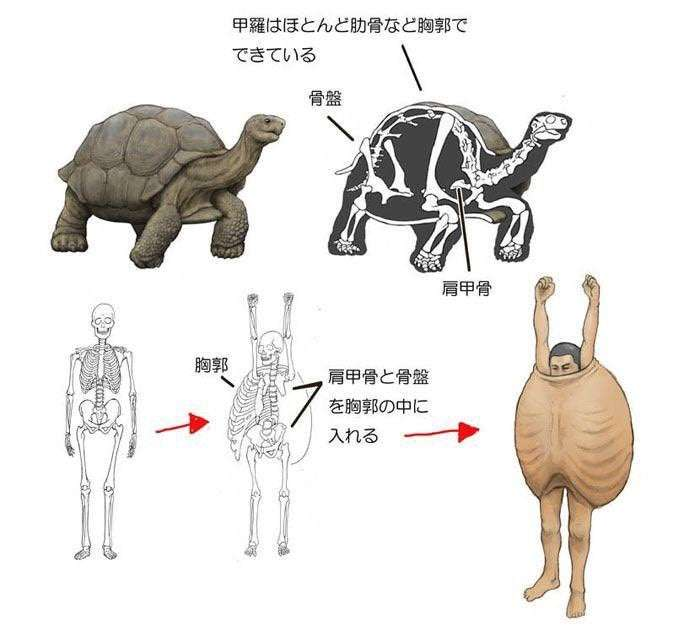
\includegraphics[trim={1cm 15cm 0 0}, clip, width=\linewidth]{mem12}
    \end{figure}
    \begin{figure}
        \centering
        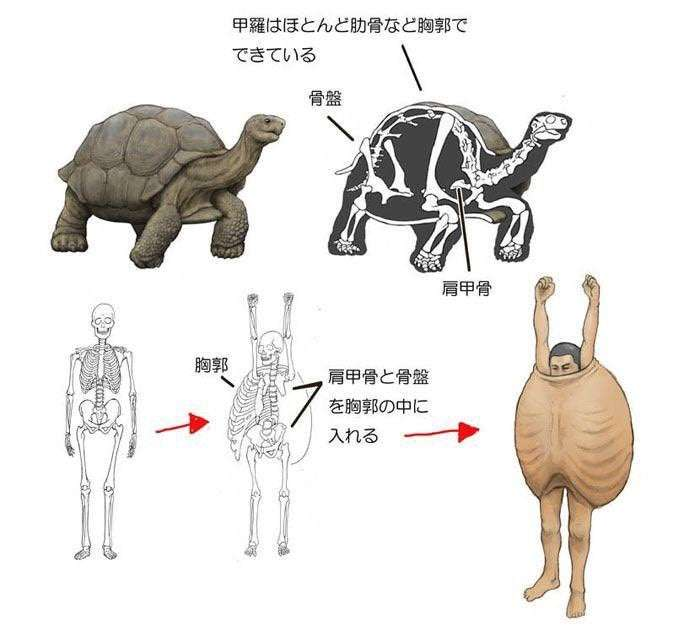
\includegraphics[trim={1cm 1cm 0 0}, clip,width=0.75\linewidth]{mem12}
    \end{figure}
    \begin{figure}
        \centering
        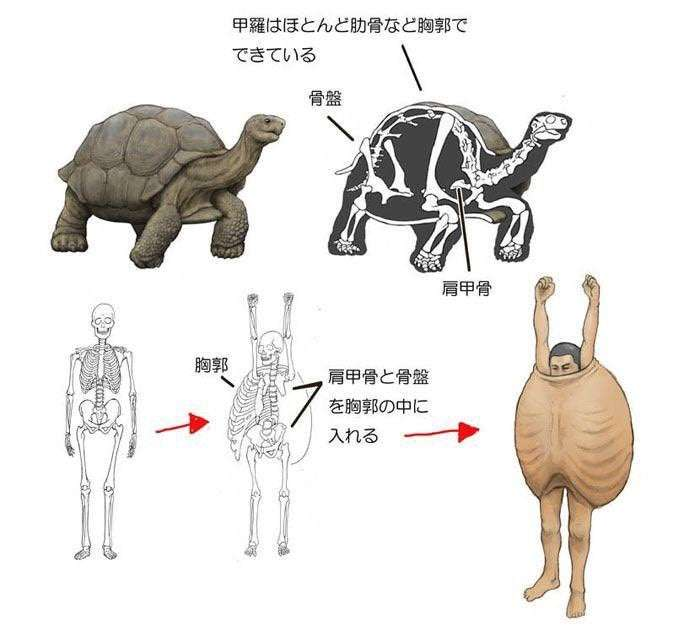
\includegraphics[trim={1cm 0cm 10cm 2cm}, clip,width=0.5\linewidth]{mem12}
    \end{figure}

    \end{columns} 
\end{frame}

\begin{frame}{I teraz możemy zacząć się bawić III}{}
    Opcja \texttt{angle}:
    \begin{itemize}
        \item \texttt{[angle = 45]}\\
        obróci o 45 stopni w dodatnim kierunku orientacji płaszczyzny
    \end{itemize}\pause
    Opcja \texttt{origin}:
    \begin{itemize}
        \item \texttt{[angle = 45, origin = tr]}\\
        obróci o 45 stopni w dodatnim kierunku orientacji płaszczyzny względem prawego górnego boku
    \end{itemize}\pause
    \texttt{\tb{rotatebox}}:
    \begin{itemize}
        \item \texttt{\tb{}rotatebox[origin = tr]\{45\}\{tekst\}}\\
        obróci o 45 stopni w dodatnim kierunku orientacji płaszczyzny względem prawego górnego roku, \rotatebox[origin = tr]{45}{o tak}
    \end{itemize}
    
\end{frame}

\section{was}

\begin{frame}{Ej, a czemu ten obrazek jest w jakimś losowym miejscu?}{}
    Musimy się cofnąć na początek (do pierwszej linijki):
    \texttt{\tb{begin\{figure\}}}
    
    Tu też są opcje:
    \begin{itemize}
        \item{} [h] (\emph{here}) -- wstaw gdzieś tutaj
        \item{} [t] (\emph{top}) -- wstaw na górze strony
        \item{} [b] (\emph{bottom}) -- wstaw na dole strony
        \item{} [p] (\emph{page}) -- wstaw na osobnej stronie
    \end{itemize}
\end{frame}

\begin{frame}{No dobra, chcę mieć obrazek tu gdzie go wstawiam}
    \begin{itemize}
        \item{} [h] (\emph{here}) -- wstaw gdzieś tutaj
        \item{} [h!]\footnote{kompilator prawdopodobnie każe ci to zrelaksować -- wpisz [ht!]} (\emph{here!}) -- wstaw gdzieś tutaj, ale pozwalam ci zignorować standardy edytorskie
        \item{} [H]\footnote{wymaga użycia paczki \texttt{\tb{usepackage\{float\}}}} (\emph{HERE, MOTYLA NOGA!}) -- wstaw DOKŁADNIE TAM gdzie jest w kodzie
    \end{itemize}
\end{frame}

\begin{frame}[fragile]{No dobra, ale ja chcę mieć tak jak w Wordzie}{}



    \begin{verbatim}
% \usepackage{wrapfig}
\begin{wrapfigure}{r}{0.3\textwidth}
    \centering
    \includegraphics[width=0.25\textwidth]{meme}
\end{wrapfigure}
    \end{verbatim}
    
    \begin{wrapfigure}[8]{r}{0.3\textwidth}
    \centering
    
\includegraphics[width=0.25\textwidth]{memy/mem5.png}
\end{wrapfigure}%
\bredzenie{82-83}
% kuć i orać w dzień zawzięcie bo zysków niema bez trudu złocisty szczęścia okręcie kołyszesz kuc my nie czekamy cudu robota to potęga ludu 
% kuć i orać w dzień zawzięcie bo zysków niema bez trudu złocisty szczęścia okręcie kołyszesz kuc my nie czekamy cudu robota to potęga ludu 
% kuć i orać w dzień zawzięcie bo zysków niema bez trudu złocisty szczęścia okręcie kołyszesz kuc my nie czekamy cudu robota to potęga ludu 
% kuć i orać w dzień zawzięcie bo zysków niema bez trudu złocisty szczęścia okręcie kołyszesz kuc my nie czekamy cudu robota to potęga ludu 
% kuć i orać w dzień zawzięcie bo zysków niema bez trudu złocisty szczęścia okręcie kołyszesz kuc my nie czekamy cudu robota to potęga ludu 


\end{frame}

\begin{frame}[fragile]{Czy ty widziałeś kiedyś Worda na oczy?}{}
    Tak, widziałem.\pause

    \begin{verbatim}
% \usepackage{wrapfig}
\begin{wrapfigure}[8]{r}{0.3\textwidth}
    \centering
    \includegraphics[width=0.25\textwidth]{meme}
\end{wrapfigure}
    \end{verbatim}
    
    \begin{itemize}[<+->]
        \item{} \texttt{[8]} -- ilość linijek które ma zawinąć, czasami poradzi sobie sam
        \item \texttt{\{r\}} -- zrób po prawej\\
        \texttt{l} -- po lewej,
        \texttt{i} -- po wewnętrznej,
        \texttt{o} -- po zewnętrznej
        \item \texttt{\{0.25\tb{}textwidth\}} -- szerokość wrapowania
        \item \texttt{[width=0.25\tb{}textwidth]} -- szerokość obrazka
        
    \end{itemize}
    
    
\end{frame}

\section{the}

\begin{frame}{No dobra, a co z pozostałymi rzeczami o których mówiłeś?}{}
\begin{columns}
\column{0.5\textwidth}
    \begin{itemize}[<+->]
        \item \texttt{\tb{caption\{\}}} -- wstawia podpis
        \item no i w sumie to tyle
    \end{itemize}
    
\column{0.5\textwidth}
\begin{figure}
    \centering
    \includegraphics[width=0.7\textwidth]{mem11}
    \caption{Podpis pod obrazkiem. Pamiętaj o \texttt{\tb{}usepackage\{polski\}} jeżeli chcesz mieć "rysunek" a nie "figure"}
    \label{fig:my_label}
\end{figure}
\end{columns}
\end{frame}

\begin{frame}[fragile]{Gdzie mi wstawi? I}

\begin{columns}
\column{0.5\textwidth}    
    \begin{verbatim}
\begin{figure}[h]
    \centering
    \caption{podpis na górze}
    
\includegraphics[...]{mem8}
\end{figure}
    \end{verbatim}
    \begin{figure}
        \centering
        \caption{Podpis na górze...}
        
\includegraphics[width=0.6\textwidth]{mem8}
        % \label{fig:my_label}
    \end{figure}
\column{0.5\textwidth}   
    \begin{verbatim}
\begin{figure}[h]
    \centering
    
\includegraphics[...]{mem8}
    \caption{podpis na dole}
\end{figure}
    \end{verbatim}
    \begin{figure}
        \centering
        
\includegraphics[width=0.6\textwidth]{mem8}
        \caption{...podpis na dole...}
        % \label{fig:my_label}
    \end{figure}
\end{columns}
\end{frame}

\begin{frame}[fragile]{Gdzie mi wstawi? II}
    \begin{verbatim}
% \usepackage[rightcaption]{sidecap}
\begin{SCfigure}[0.5][h]
    \centering
    \caption{podpis po prawej}
    
\includegraphics[width=0.6\textwidth]{mem8}
\end{SCfigure}\end{verbatim}
    \begin{figure}
        \centering
        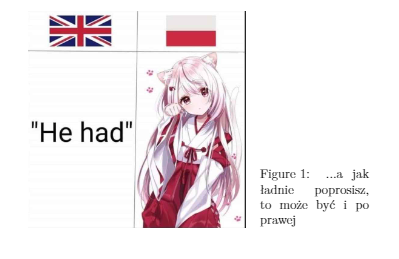
\includegraphics[width=0.5\textwidth]{memy/Zrzut ekranu 2024-12-06 090913.png}
        \caption{Musicie mi uwierzyć że to działa, jest trzecia w nocy, wyskakują mi \emph{dziwne błędy}, a przed przedawkowaniem środków odurzających ratuje mnie tylko doświadczenie}
        % \label{fig:my_label}
    \end{figure}
\end{frame}

\begin{frame}{Czym się różni \texttt{caption} od \texttt{label}?}{}
    \begin{itemize}[<+->]
        \item W zasadzie to wszystkim:
        \item \texttt{caption} to podpis pod rysunkiem, dla czytelników
        \item \texttt{label} to znacznik do odwoływania się, widziany tylko w kodzie (przez autora)
    \end{itemize}
\end{frame}

\begin{frame}[fragile]{To jak się korzysta z \texttt{label}a?}{}
\begin{verbatim}
\begin{figure}
    \centering
    
\includegraphics[width=0.5\textwidth]{memy/mem4.png}
    \caption{Jakiś śmieszny podpis}
    \label{fig:andrzej}
\end{figure}

\bredzenie{171}
Zobacz rysunek \ref{fig:andrzej}.
\bredzenie{172}
\end{verbatim}
\end{frame}

\begin{frame}{No i co, potrafisz tak zrobić w Wordzie?}
    \begin{figure}
        \centering
        
\includegraphics[width=0.5\textwidth]{memy/mem4.png}
        \caption{W tym żarcie chodzi o to, że słowo \texttt{latex} ma dwa znaczenia}
        \label{fig:zart}
    \end{figure}
    {\tiny \bredzenie{171} \textbf{Jak wspomniałem w poprzednim mailu, na rysunku \ref{fig:zart}...}  \bredzenie{172}}
\end{frame}

\section{\LaTeX}

\begin{frame}[fragile]{Multiplikacja}{}
    % Subfigures:
    \begin{verbatim}
\begin{figure}
    \centering
    \begin{subfigure}{0.5\textwidth}
        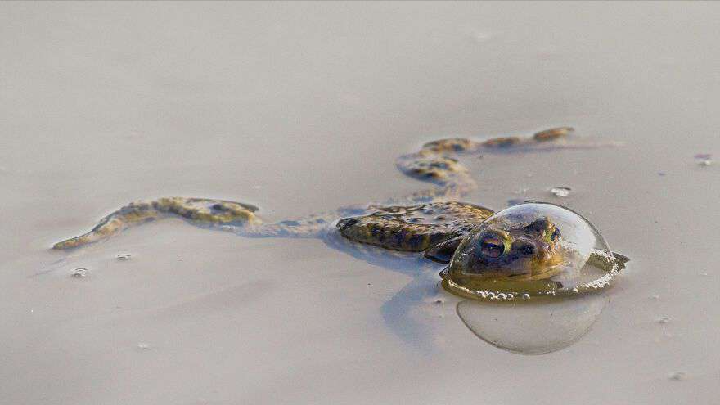
\includegraphics[width=\textwidth]{mem6}
        \caption{Śmieszny mem}
        \label{smieszny}
    \end{subfigure}
    \begin{subfigure}{0.5\textwidth}
        
\includegraphics[width=\textwidth]{mem7}
        \caption{Nieśmieszny mem}
        \label{niesmieszny}
    \end{subfigure}
    \caption{Przykłady memów}
    \label{memy}
\end{figure}
    \end{verbatim}
\end{frame}


\begin{frame}[fragile]{Multiplikacja}{}
    % Subfigures:
    % \begin{verbatim}
\begin{figure}
    \centering
    \begin{subfigure}[c]{0.45\textwidth}
        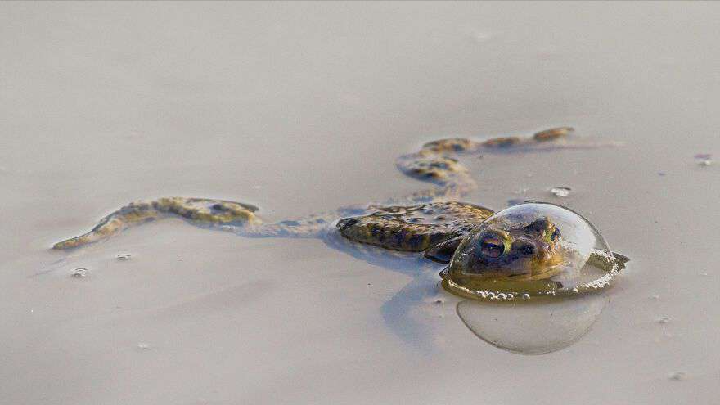
\includegraphics[width=\textwidth]{mem6}
        \caption{Śmieszny mem}
        \label{smieszny}
    \end{subfigure}
    \begin{subfigure}[c]{0.45\textwidth}
        
\includegraphics[width=\textwidth]{mem7}
        \caption{Nieśmieszny mem}
        \label{niesmieszny}
    \end{subfigure}
    \caption{Przykłady żabów}
    \label{memy}
\end{figure}

Jak można sprawdzić, można \texttt{\tb{ref}}ować zarówno do obrazka \ref{smieszny}, do obrazka \ref{niesmieszny}, jak i do całego obrazka \ref{memy}.

    % \end{verbatim}
\end{frame}

\begin{frame}{A czy można robić obrazki samemu?}{}
\setbeamercovered{invisible}
    \pause
    \begin{figure}
    \begin{tikzpicture}
        \duck[torch=gray!70!brown, tshirt=blue!10!black, santa=red!80!black, ribbon=gray, bowtie=blue!50!white];
         \fill[cyan!20!white] (-1.6,1.8) ellipse (1.8 and 0.5);
  \fill[cyan!20!white] (-0.2,1.54) -- (0.2,1.35) -- (0.0,1.6) -- cycle;
	\node at (-1.6,1.8) {O tym będzie jutro};
    \end{tikzpicture}
    \caption{sobota, 15:50}
    \end{figure}
    
\end{frame}



\end{document}
